% !TEX root = ../main.tex
\section{윤리 승인 증명서}
\label{ch:appendix-ethics}

이 연구는 누구나 볼 수 있는 공개 블록체인 자료만 써요. 그리고 사람을 연구 참여자로 두지 않아요(\ref{sec:ethics}절). 남아프리카 대학교(Unisa) 과학·공학·기술 대학(CSET) 컴퓨팅 학부의 연구 윤리 심사 위원회가 이 연구를 위험이 낮은 연구로 심사했고, 2026년 11월 9일에 5년 동안의 윤리 승인(연구가 윤리 기준을 지킨다는 허가)을 주었어요(참조 번호 18316). 이 부록의 마지막 두 쪽에 위원회가 발급한 증명서를 그대로 옮겨 실어요.

% 원본: Figures/ethics-clearance.pdf는 위원회가 발급한 증명서(두 쪽, 참조 번호 18316)예요.
% The page is ended here by hand: pdfpages holds every float that is still waiting until
% after the pages it inserts, which would put the last table of the appendix behind the certificate.
% Each page is scaled and moved up so that its frame ends above the page number of the thesis.
\clearpage
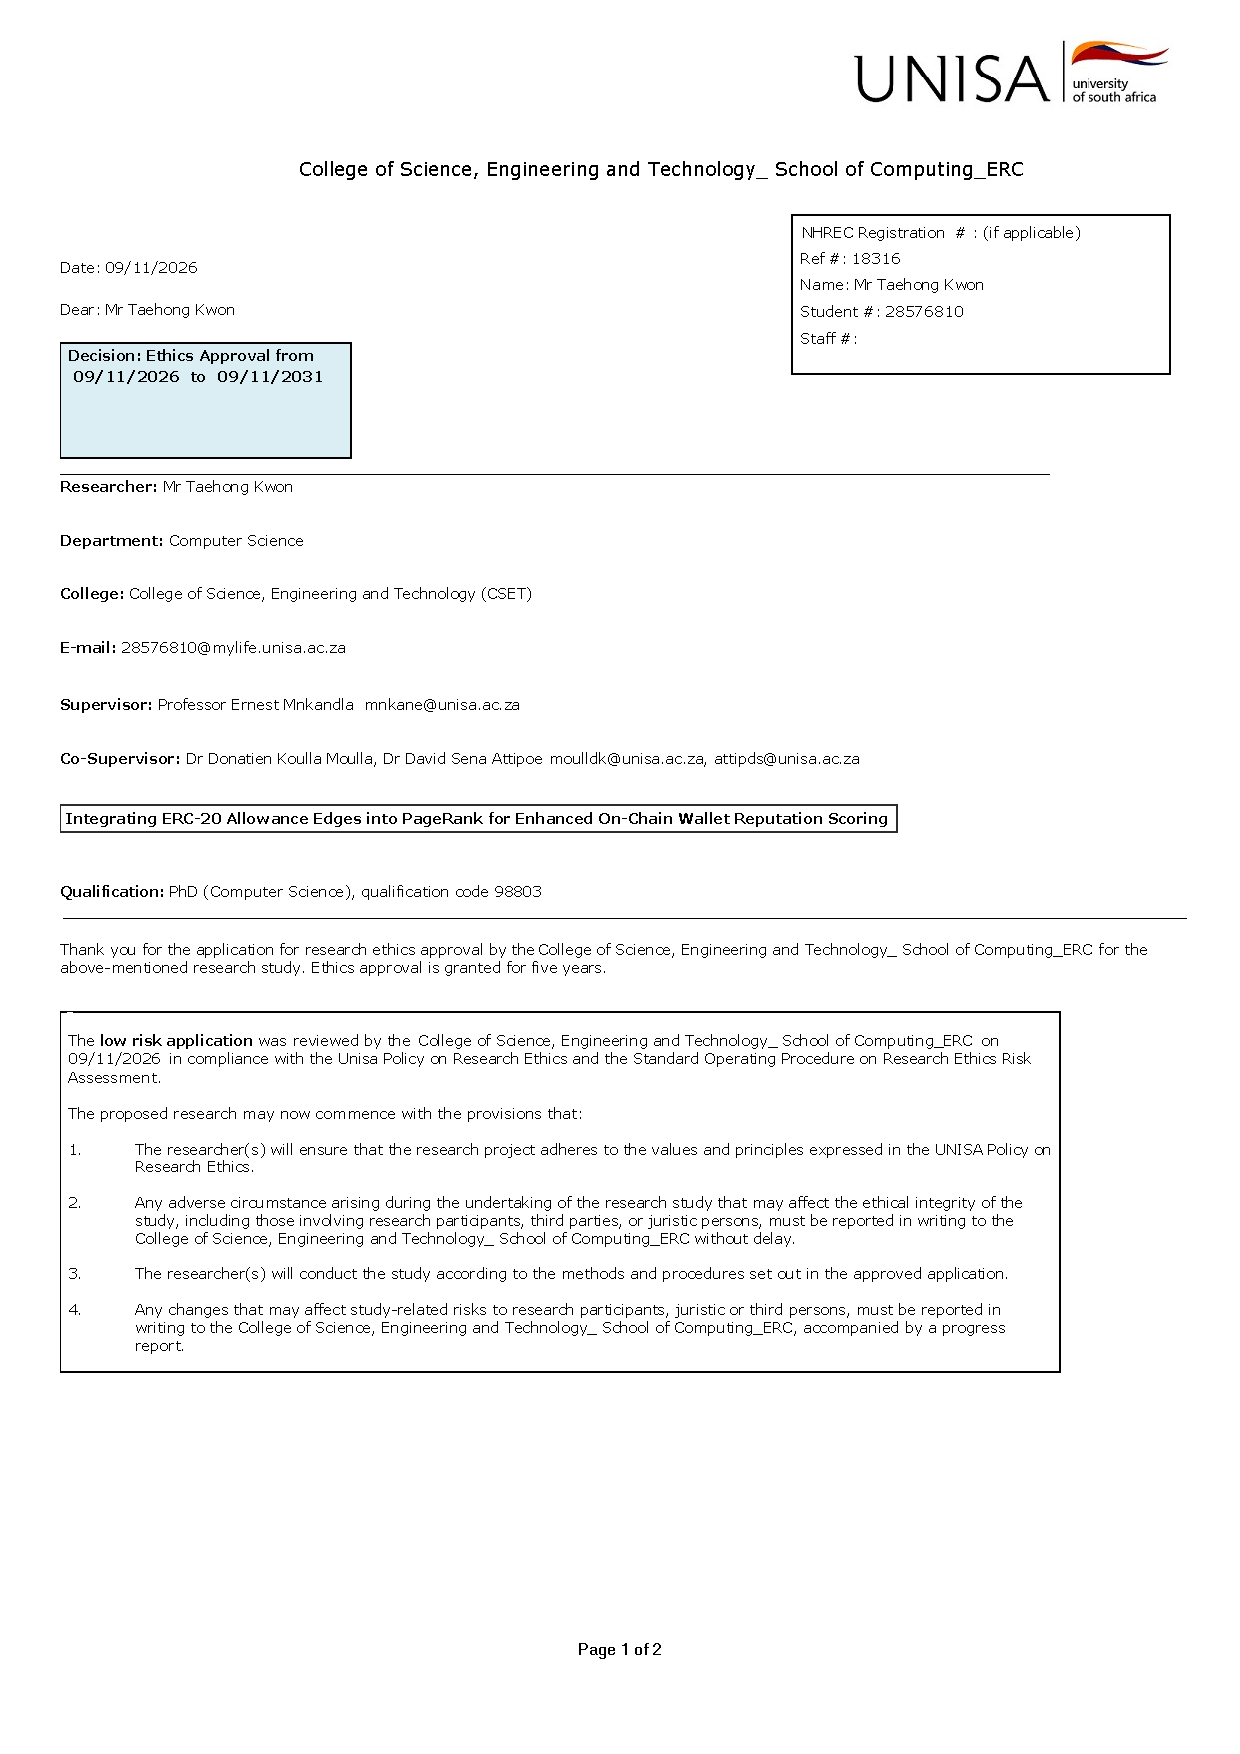
\includepdf[pages=1-2,scale=0.80,offset=0 16mm,frame=true,pagecommand={\thispagestyle{plain}}]{Figures/ethics-clearance.pdf}
